\documentclass[usepdftitle=false]{beamer}

\mode<presentation> {
  \usetheme{Madrid}
\colorlet{beamer@blendedblue}{green!40!black}
  \setbeamercovered{invisible}
}

\usepackage[english]{babel}
\usepackage[utf8]{inputenc}
\usepackage{times}
\usepackage[T1]{fontenc}

\usepackage{listings}
\usepackage{xcolor}
\usepackage{algorithm}
\usepackage{algpseudocode}
\usepackage{booktabs}
\usepackage{graphicx}
\usepackage{hyperref}
\usepackage{multicol}
\usepackage{xspace}
\usepackage{tikz}

% Define Lean code style
\lstdefinestyle{leanstyle}{
  language=Lisp,
  basicstyle=\small\ttfamily,
  keywordstyle=\color{blue},
  commentstyle=\color{gray},
  stringstyle=\color{red},
  breaklines=true,
  showstringspaces=false
}

% Commands
\newcommand{\sal}{\textsc{Sal}\xspace}
\newcommand{\fstar}{F$^{\star}$\xspace}
\newcommand{\F}[1]{\mathsf{#1}}
\newcommand{\M}[1]{\mathcal{#1}}

\title[\sal: Multi-modal Verification]{
  \sal: Multi-modal Verification of Replicated Data Types
}

\author{Pranav R \and Vimala S \and KC Sivaramakrishnan}

\institute{
  Indian Institute of Technology, Madras
}


\subject{Verification of Replicated Data Types}

\begin{document}

\begin{frame}
  \titlepage
\end{frame}



% ===========================================================================================
\section{Introduction: Replication in Practice}
% ===========================================================================================

\begin{frame}
  \frametitle{Local-First Collaboration}
  \begin{itemize}[<+->]
    \item Users work offline, synchronize when connectivity returns
    \item Replicas evolve independently, must merge accurately
    \item Example: Shared documents, collaborative editors
  \end{itemize}
  \vspace{0.5cm}
  \centering
  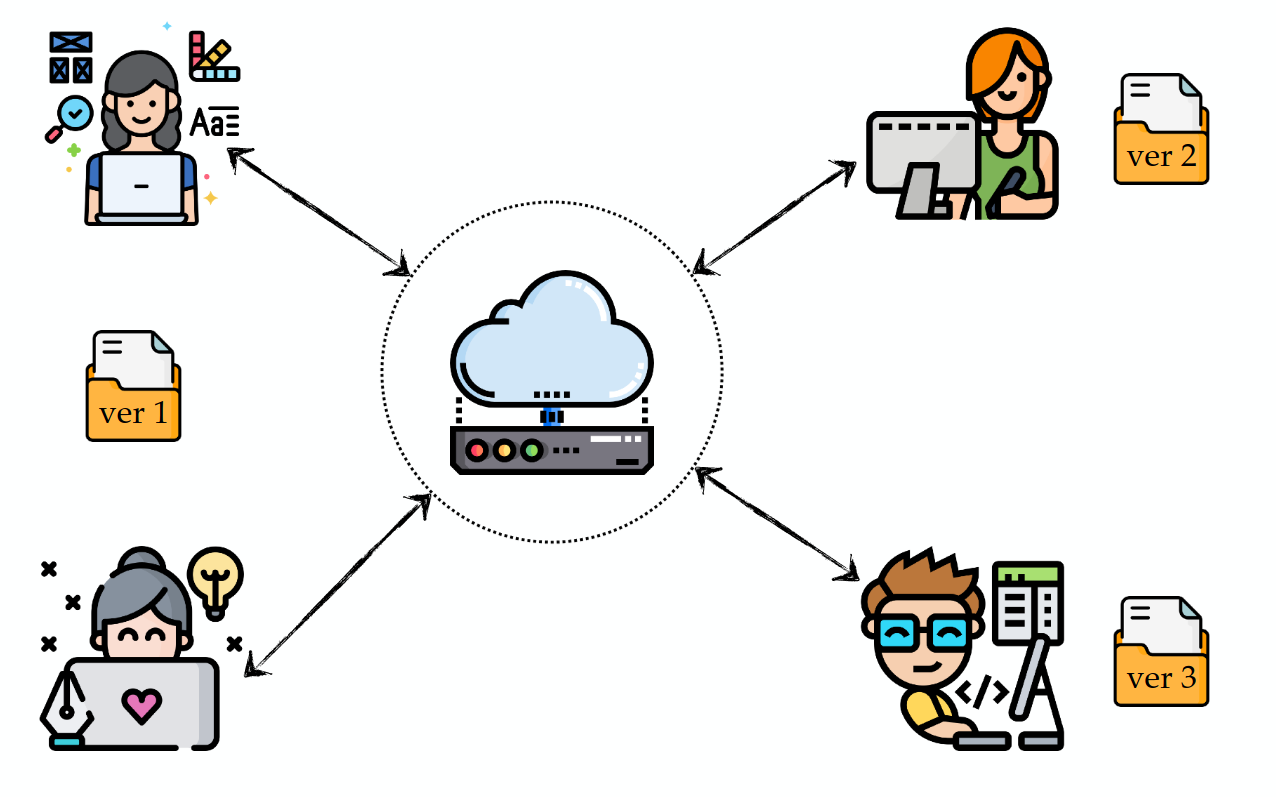
\includegraphics[width=0.6\textwidth]{Pictures/local_first_collaboration_diagram.png}

  
  \textbf{Challenge:} How do we ensure correctness when states diverge?
\end{frame}

\begin{frame}
  \frametitle{CRDTs and MRDTs: Building Blocks}
  \begin{description}
    \item[CRDT] Conflict-Free Replicated Data Type
      \begin{itemize}[<+->]
        \item Deterministic two-way merge
        \item Requires tombstones
      \end{itemize}
    
    \vspace{0.2cm}
    \item[MRDT] Mergeable Replicated Data Type
      \begin{itemize}[<+->]
        \item Three-way merge (like Git)
        \item More compact representations (e.g., $O(1)$ counter state vs $\Omega(n)$ in CRDTs due to tombstones)
      \end{itemize}
  \end{description}
  
  \vspace{0.2cm}
  \centering
  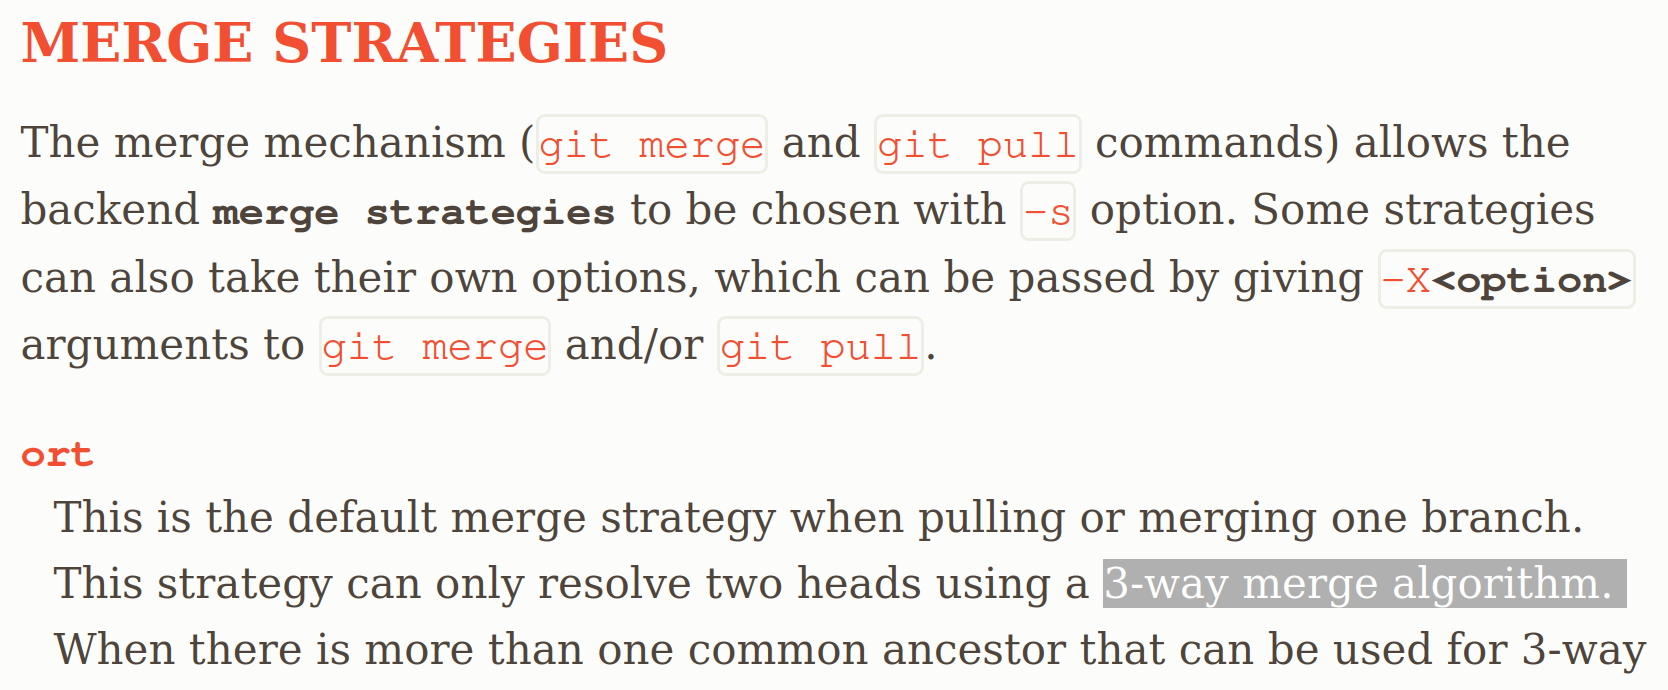
\includegraphics[width=0.6\textwidth]{Pictures/git_merge.png}
  
  \small\textit{Three-way merge model in git (git-ort)}
\end{frame}

\begin{frame}
  \frametitle{Example: Increment-Only Counter MRDT}
  
  \begin{columns}
    \column{0.5\textwidth}
    \small
    \begin{tabular}{ll}
      \toprule
      \textbf{Component} & \textbf{Definition} \\
      \midrule
      State & $\Sigma = \mathbb{N}$, $\sigma_0 = 0$ \\
      Initial & $\sigma_0 = 0$ \\
      Update & $\F{do}(\sigma, \ldots, \F{inc}) = \sigma + 1$ \\
      Merge & $\F{merge}(\sigma_{lca}, \sigma_1, \sigma_2)$ \\
           & $\quad = \sigma_{lca} + (\sigma_1 - \sigma_{lca})$ \\
           & $\quad \quad + (\sigma_2 - \sigma_{lca})$ \\
      Conflicts & $\F{rc} = \emptyset$ (none) \\
      \bottomrule
    \end{tabular}
    
    \column{0.5\textwidth}
    \centering
    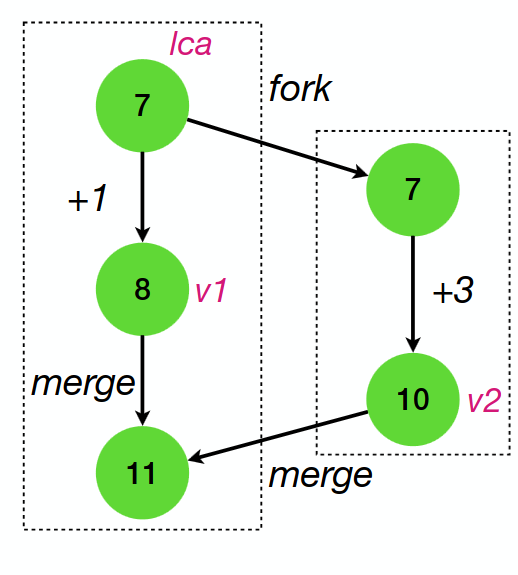
\includegraphics[width=0.95\textwidth]{Pictures/inc_only_counter_mrdt.png}
    
    \vspace{0.3cm}
    \small\textit{Three-way merge after concurrent increments}
  \end{columns}
\end{frame}


% ===========================================================================================
\section{The Verification Problem}
% ===========================================================================================

\begin{frame}
  \frametitle{Why Verification Matters}
  
  \begin{quote}
    \textit{Designing correct replicated data types is challenging.}
  \end{quote}
  
  \vspace{0.2cm}
  \centering
  
  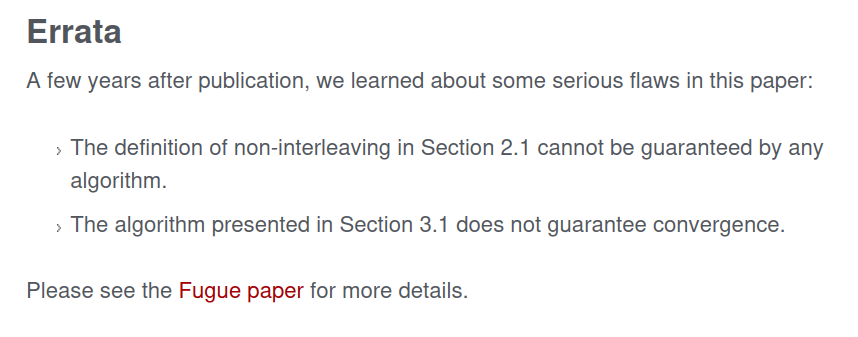
\includegraphics[width=0.7\textwidth]{Pictures/errata_kleppman.png}
  
  \small\textit{RGA anomaly: The definition of non-interleaving in that paper cannot be satisfied by any algorithm}
  
  \vspace{0.3cm}
  
  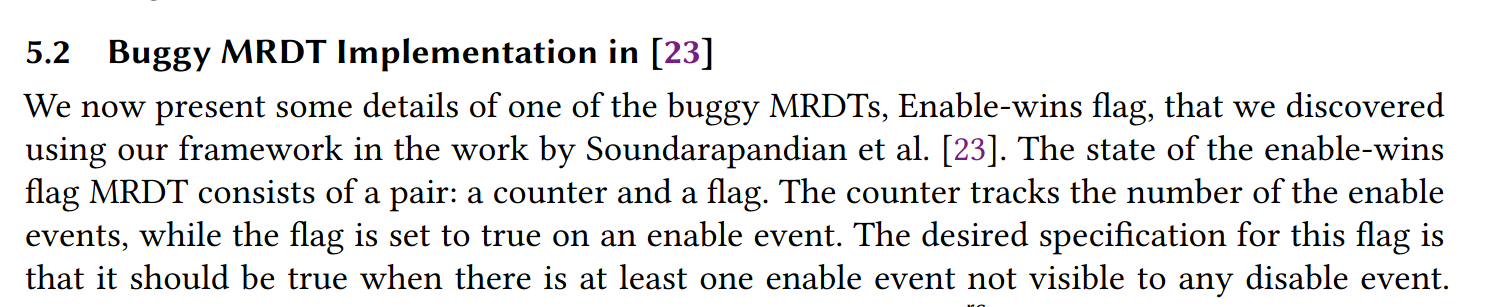
\includegraphics[width=0.7\textwidth]{Pictures/errata_vimala.png}
  
  \small\textit{Enable-wins flag bug: Incorrect merge logic allows disabled state to incorrectly become enabled}
\end{frame}

\begin{frame}
  \frametitle{Replication-Aware (RA) Linearizability}
  
  \begin{block}{Definition}
    RA linearizability relates replica executions to a sequential explanation of updates, ensuring that:
    \begin{itemize}[<+->]
\item The state at any replica during any execution must be achievable by applying a sequence (or linearization) of the
update operations visible to the replica.
\item This linearization should obey the user-specified
conflict resolution policy for concurrent operations, and the local replica order for non-concurrent
operations.
\item Our definition of RA-linearizability allows viewing the state of an MRDT replica as a sequence
of update operations applied on the initial state, thus abstracting over the merge function and how
it handles concurrent operations. 
    \end{itemize}
  \end{block}
  
  \vspace{0.3cm}
  Neem reduced RA-linearizability to 24 verifiable conditions (VCs)
\end{frame}

% ===========================================================================================
\section{Verification with F* and its Limitations}
% ===========================================================================================

\begin{frame}
  \frametitle{Prior Work: Neem in \fstar}
  
  \begin{block}{Strengths}
    \begin{itemize}[<+->]
      \item SMT-aided automation for RA linearizability
      \item Formal reduction to 24 verification conditions
      \item Practical verification of CRDTs and MRDTs
    \end{itemize}
  \end{block}
  
  \vspace{0.3cm}
  \begin{block}{The Problem: Trust in SMT Solvers}
    \begin{itemize}[<+->]
      \item SMT-centric workflows are opaque when automation fails
      \item Failed VC provides little actionable feedback
      \item Relies on external solver $\rightarrow$ larger trusted computing base (TCB)
      \item Debugging requires manual proof-debugging workflow
      \item SMT proofs are brittle to small changes
    \end{itemize}
  \end{block}
\end{frame}

% ===========================================================================================
\section{Solution: SAL Framework}
% ===========================================================================================

\begin{frame}
  \frametitle{\sal Overview}
  
  \begin{block}{A Multi-Modal Workflow for RA Linearizability in Lean}
    \begin{enumerate}[<+->]
      \item \textbf{Kernel-checkable automation} with proof reconstruction
      \item \textbf{SMT-aided automation} when needed (fallback)
      \item \textbf{AI-assisted interactive theorem proving} for remaining obligations
      \item \textbf{Counterexample generation} and visualization
      \item \textbf{The grind tool in Lean offers kernel-checkable proofs}

    \end{enumerate}
  \end{block}
  
  \begin{center}
    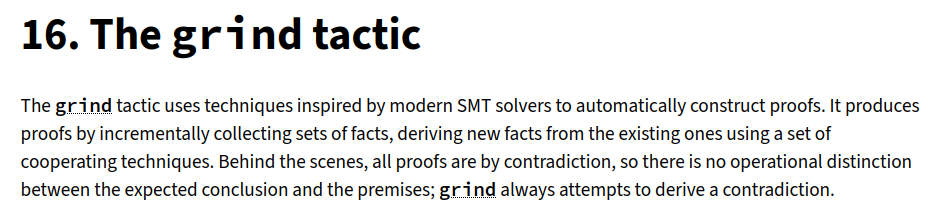
\includegraphics[width=0.45\textwidth]{Pictures/grind_desc_1.png}\hspace{0.5cm}
    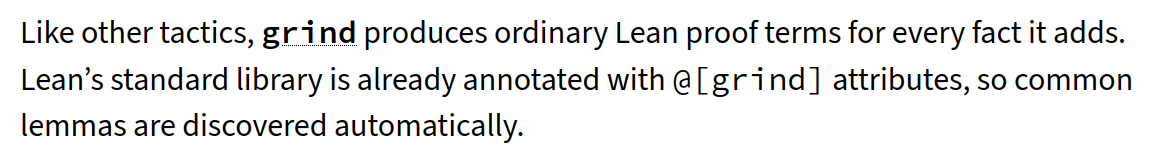
\includegraphics[width=0.45\textwidth]{Pictures/grind_desc_2.png}
  \end{center}
\end{frame}


\begin{frame}[fragile]
  \frametitle{Key Design: Data Structures for Automation}
  
  \textbf{Challenge:} Lean's standard library optimizes for manual proofs, not automation
  
  \vspace{0.3cm}
  \begin{block}{Custom Set and Map Interfaces}
    \small
    \begin{lstlisting}[style=leanstyle,basicstyle=\tiny\ttfamily]
-- Set: Boolean-valued membership
@[simp]
abbrev set (a:Type) [DecidableEq a] := a -> Bool

@[simp, grind]
def union {a:Type} [DecidableEq a] (s1 s2 : set a) : set a :=
(fun x => s1 x || s2 x)

@[simp, grind]
def intersection {a:Type} [DecidableEq a] (s1 s2: set a) : set a :=
(fun x => s1 x && s2 x)

-- Map: Explicit domain
structure map (key:Type) [DecidableEq key] (value:Type) where
  (mappings: key -> value) (domain: set key)
    \end{lstlisting}
  \end{block}
  
  \vspace{0.2cm}
  \textbf{Automation-friendly:} All operations are directly computable!
\end{frame}

% ===========================================================================================
\section{Counterexample Generation and Visualization}
% ===========================================================================================

\begin{frame}
  \frametitle{The Enable-Wins Flag Bug}
  
  \begin{block}{Specification}
    A shared boolean flag with concurrent enable/disable operations.
    When enable and disable are concurrent, \textbf{enable wins}.
  \end{block}
  
  \vspace{0.3cm}
  \textbf{Naive Implementation Bug:}
  \begin{itemize}[<+->]
    \item Track concurrent enables with a counter
    \item Use counter to decide flag state after merge
    \item \textbf{Problem:} Enables followed by disables on each replica still show as enabled!
  \end{itemize}
\end{frame}

\begin{frame}[fragile]
  \frametitle{RA-Linearizability Verification Condition (VC)}
  
  \small
  \begin{lstlisting}[style=leanstyle, basicstyle=\tiny\ttfamily, breaklines=true]
theorem inter_right_1op (l: concrete_st) (a: concrete_st) 
  (b: concrete_st) (o1: op_t) (ob: op_t) (ol: op_t) (o: op_t) :
  rc ob ol = rc_res.Fst_then_snd /\ get_rid ob != get_rid ol /\
  (~ (rc o ob = rc_res.Either) \/ (rc o ol = rc_res.Fst_then_snd)) /\
  distinct_ops o1 ob /\ distinct_ops o1 ol /\ 
  distinct_ops o1 o /\ distinct_ops ob ol /\ 
  distinct_ops ob o /\ distinct_ops ol o /\
  get_rid o != get_rid ol /\
  eq (merge (do_ l ol) (do_ (do_ a ol) o1) 
     (do_ (do_ b ob) ol))
     (do_ (merge (do_ l ol) (do_ a ol) 
     (do_ (do_ b ob) ol)) o1)
  ->
  eq (merge (do_ l ol) (do_ (do_ a ol) o1) 
     (do_ (do_ (do_ b o) ob) ol))
     (do_ (merge (do_ l ol) (do_ a ol) 
     (do_ (do_ (do_ b o) ob) ol)) o1)
  \end{lstlisting}
  
  \vspace{0.2cm}
  \small Conditions ensure interleaving property: operations commute correctly across merge boundaries
\end{frame}


\begin{frame}
  \frametitle{Concrete Counterexample: Enable-Wins Flag Execution}
  
  \centering
  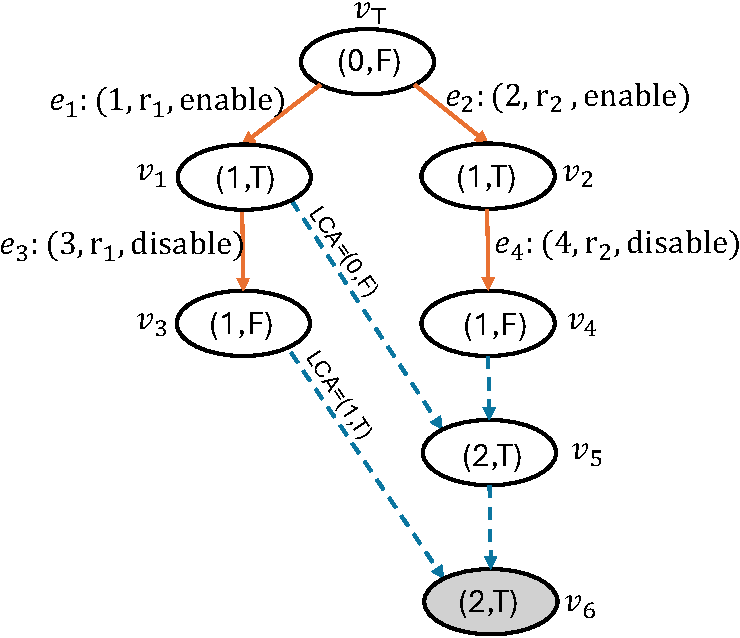
\includegraphics[width=0.6\textwidth]{../SAL___Multi_modal_Verification_of_Replicated_Data_Types/ewflag-counterexample.pdf}
  
  \small
  \vspace{0.2cm}
  \textit{Automatic counterexample shows: both replicas disable the flag ($v_3, v_4$), yet merge produces (2, true)---flag is incorrectly enabled!}
\end{frame}



\begin{frame}[fragile]
  \frametitle{Automated Counterexample Discovery}
  
  \textbf{Approach:} Use Plausible (property-based testing for Lean)
  
  \begin{block}{Process}
    \begin{enumerate}[<+->]
      \item Express VCs as \textbf{decidable propositions}
      \item Plausible generates random test inputs
      \item Check whether VC holds for each input
      \item When violation found: report the failing input
      \item Uses machinery from the Loom work from VERSE lab
    \end{enumerate}
  \end{block}
  
  \vspace{0.3cm}
  Example failing input:
  \begin{lstlisting}[style=leanstyle]
(disable, (enable, (enable, (disable, (0, false)))))
  \end{lstlisting}
\end{frame}

\begin{frame}[fragile]
  \frametitle{Plausible: Making VCs Testable}
  
  \begin{enumerate}[<+->]
    \item \textbf{Proving Precondition Decidable} by upper bounding the values of the operations and counters, 
    and subsequently using \texttt{decidable\_by\_nat\_upperbound}
    
    \begin{center}
      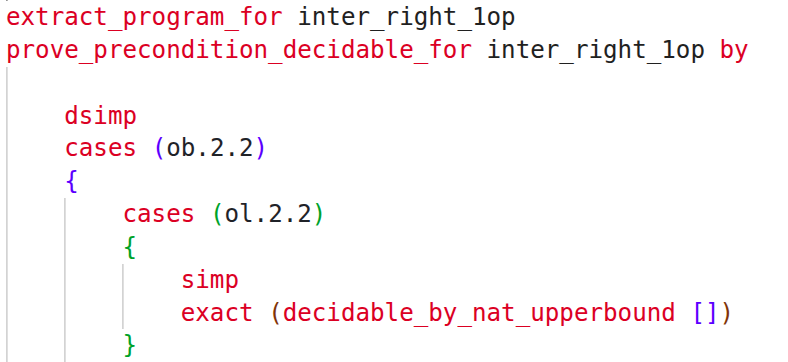
\includegraphics[width=0.5\textwidth]{Pictures/precond_decidable.png}
    \end{center}
    
    \vspace{0.2cm}
    \item \textbf{Proving Postcondition Decidable} again by using \texttt{decidable\_by\_nat\_upperbound}
    
    \begin{center}
      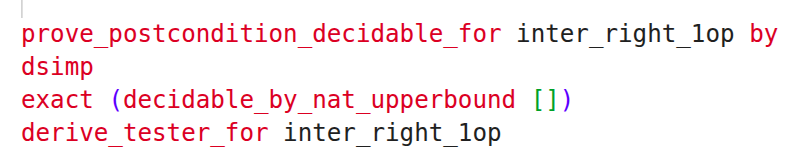
\includegraphics[width=0.5\textwidth]{Pictures/postcond_decidable.png}
    \end{center}
  \end{enumerate}
\end{frame}

\begin{frame}[fragile]
  \frametitle{Plausible: Running the Elaborator}
  
  \begin{enumerate}[<+->]
    \setcounter{enumi}{2}
    \item \textbf{Running the Elaborator in Monadic Framework}\\
    Running an elaborator in a monadic framework to generate and display the counterexample
  \end{enumerate}
  
  \vspace{0.3cm}
  \centering
  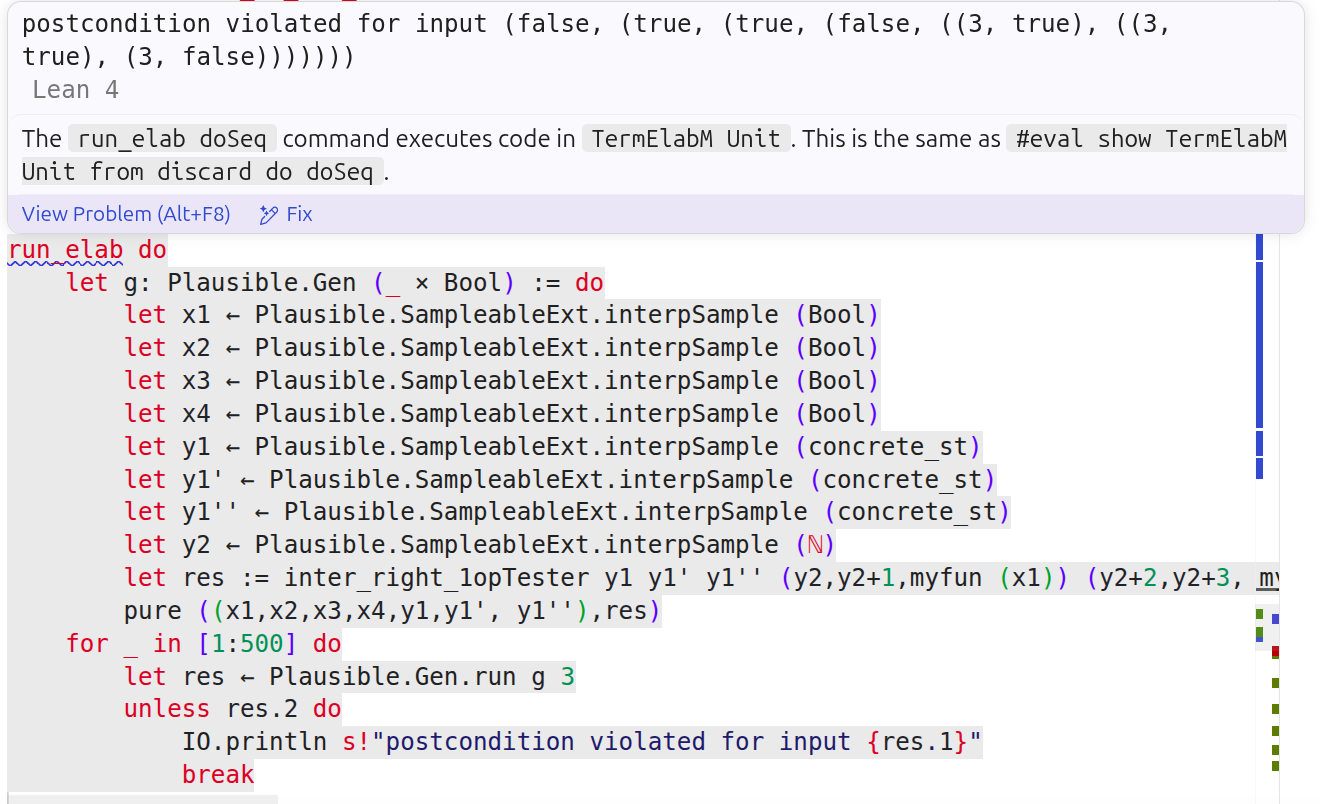
\includegraphics[width=0.85\textwidth]{Pictures/running_plausible.png}
\end{frame}

\begin{frame}
  \frametitle{Execution Trace Visualization in Lean}
  
  \begin{block}{The Challenge}
    Raw counterexample is hard to understand---why does it fail?
  \end{block}
  
  \vspace{0.3cm}
  \textbf{Solution:} ProofWidgets-based execution trace visualizer
  
  \begin{itemize}[<+->]
    \item Instrument $\F{do}$ and $\F{merge}$ operations
    \item Record intermediate states and operations
    \item Produce step-by-step execution trace
    \item Interactive visualization in Lean
  \end{itemize}
  
  \vspace{0.2cm}
  \textit{Transforms opaque proof failures into tangible test cases}
\end{frame}


\begin{frame}
  \frametitle{Enable-Wins Flag: Verification Conditions}
  
  \centering
  \small
  \begin{tabular}{cc}
    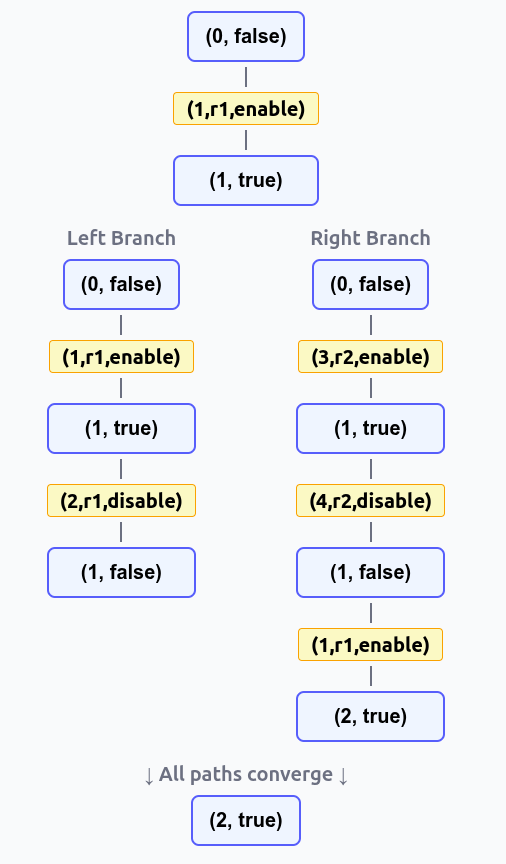
\includegraphics[width=0.3\textwidth]{../SAL___Multi_modal_Verification_of_Replicated_Data_Types/EN_wins_flag_LHS.png} &
    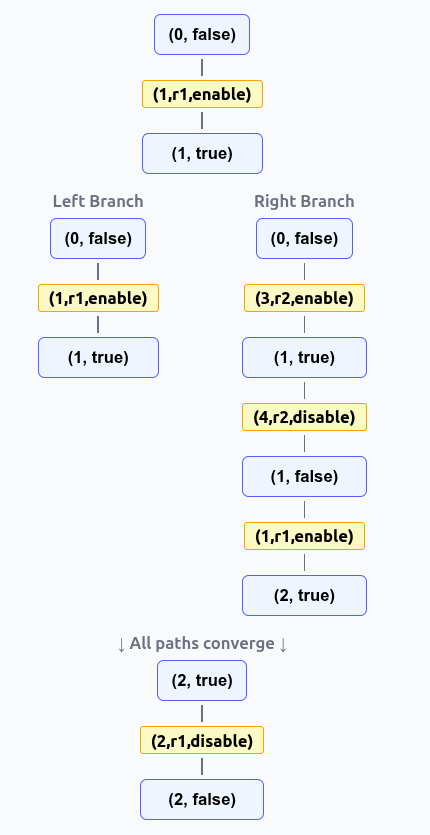
\includegraphics[width=0.3\textwidth]{../SAL___Multi_modal_Verification_of_Replicated_Data_Types/EN_wins_flag_RHS.png} \\
    \small LHS (merge result) & \small RHS (expected after linearization)
  \end{tabular}
  
\end{frame}

% ===========================================================================================
\section{Agentic Framework}
% ===========================================================================================

\begin{frame}
  \frametitle{Multi-Modal Verification: Agentic Framework}
  
  \begin{block}{Stepping Back}
    \sal is more than tactics—it's a collaborative verification workflow:
  \end{block}
  
  \vspace{0.3cm}
  \begin{itemize}[<+->]
    \item \textbf{Kernel automation:} Handles routine reasoning
    \item \textbf{SMT when needed:} For harder goals
    \item \textbf{AI assistance:} Proofs from Aristotle and Claude
    \item \textbf{Developer:} Makes informed decisions based on counterexample and proof strategies given by LLMs
  \end{itemize}
\end{frame}


\begin{frame}
  \frametitle{AI-Assisted Verification: Agentic-Driven Commits}
  
  \centering
  \begin{figure}
    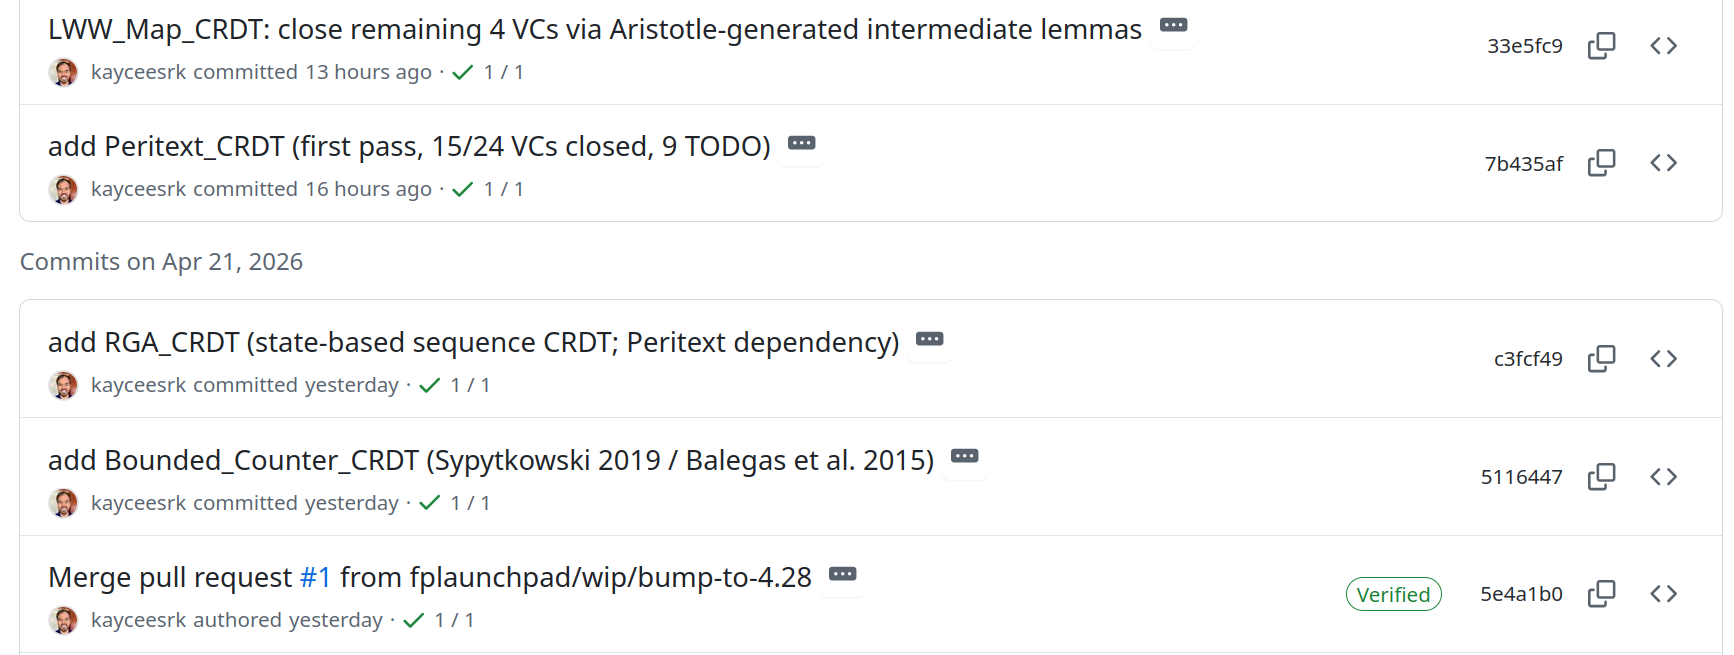
\includegraphics[width=\textwidth]{Pictures/kc_commits.png}
  \end{figure}
\end{frame}

\begin{frame}
  \frametitle{AI-Assisted Verification: NodeJs Interactive Simulations }
  
  \centering
  \begin{figure}
    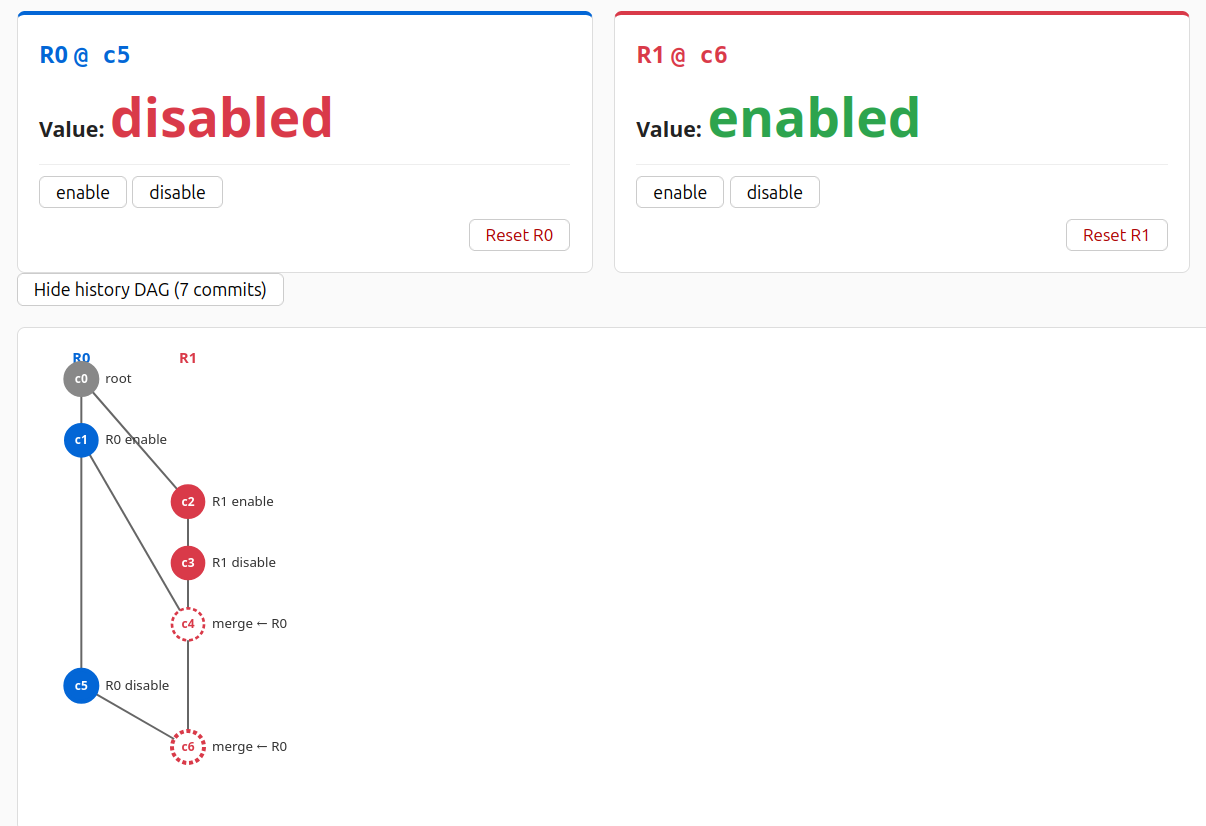
\includegraphics[width=0.9\textwidth]{Pictures/npm_visualization.png}
  \end{figure}
\end{frame}


\begin{frame}
  \frametitle{AI-Assisted Verification: Verification Status}
  
  \centering
  \begin{figure}
    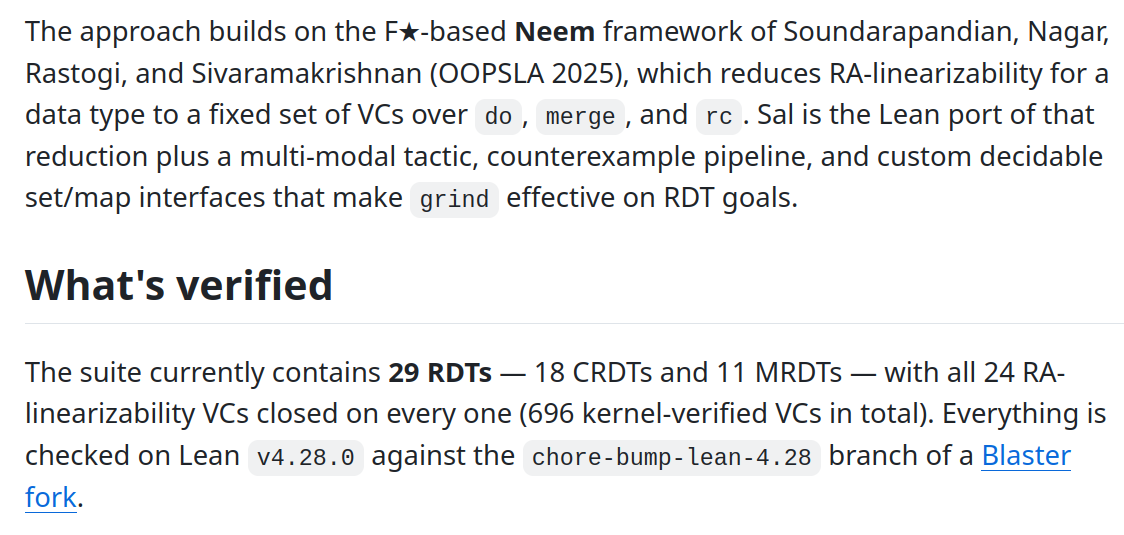
\includegraphics[width=\textwidth]{Pictures/verified_status.png}
  \end{figure}
\end{frame}


% ===========================================================================================
\section{Evaluation and Results}
% ===========================================================================================


\begin{frame}
  \frametitle{Results Table}
  
  \small
\begin{table}[t]
\caption{Number of VCs discharged by the \sal tactic (total VCs = 24 per RDT). DG refers to $\F{dsimp + grind}$, and LB refers to $\F{lean-blaster}$. }
\label{tab:results_1}
\centering
\footnotesize
\begin{tabular}{lcccc}
\toprule
\textbf{RDT} &
\textbf{DG} &
\textbf{LB} &
\textbf{ITP (Aristotle)} &
\textbf{Time (s)} \\
\midrule
Increment-only counter MRDT    & 24 & 0  & 0 & 0.7  \\
PN-counter MRDT                & 24 & 0  & 0 & 2.7  \\
OR-set MRDT                    & 3  & 21 & 0 & 17.3 \\
Enable-wins flag MRDT   & 9  & 14 & 0 & 34.2 \\
Efficient OR-set MRDT          & 2  & 22 & 0 & 14.4 \\
Grows-only set MRDT            & 24 & 0  & 0 & 0.3  \\
Grows-only map MRDT            & 22 & 0  & 2 & 25.8 \\
Replicated growable array MRDT & 15 & 9  & 0 & 3.9  \\
Multi-valued register MRDT     & 24 & 0  & 0 & 0.3  \\
Increment-only counter CRDT    & 24 & 0  & 0 & 1.5  \\
PN-counter CRDT                & 16 & 2  & 6 & 99.5 \\
Multi-valued register CRDT     & 24 & 0  & 0 & 0.7  \\
OR-set CRDT                    & 4  & 19 & 1 & 34.7 \\
\bottomrule
\end{tabular}
\end{table}
\end{frame}

\begin{frame}
  
  \vspace{0.5cm}
  \centering
  \Large\textbf{Thank you!}
  
  \vspace{0.3cm}
  \normalsize Questions?
\end{frame}

\end{document}
